\documentclass[11pt]{article}
\usepackage[margin=0.7in]{geometry}
\newcommand{\ts}{\textsuperscript}
%Gummi|065|=)
\date{}

%%%%% Please Check this section %%%%%
\title{Table of Contents}

\usepackage{graphicx}
\begin{document}

%% This is Final Report for MSE 110
%	Must be single spaced which I think it is right
%	Printed on BOTH pages
%	Include a listing of the program 
%	Submit all the project files on canvas
%	Use the cover paper provided on canvas (I made the file)
%	include a link to the project demonstration video (Maybe use youtube or google drive

%% Structure of the report (Refer to the document 'Final Project Report Instruction.pdf')
%	Progress section
%	Mechanical Design
%	Software Design 


\maketitle

\tableofcontents

\newpage


\section{Progress Report}
\subsection{1\ts{st} Iteration}

Should be achieved by:
\subsection{2\ts{nd} Iteration}

Should be achieved by:
\subsection{3\ts{rd} Iteration}

Should be achieved by:



\newpage
\section{Mechanical Design of MazeBot}

\subsection{First Iteration}
\textbf{Goals:}
\begin{itemize}
\item Accurate movement
\end{itemize}
\underline{\textbf{Mechanical Drawing}}\\

\underline{\textbf{Observations \& Measurements}}\\\\
\textbf{Structural Integrity of the Drive System}\\
In order for more accurate movement, we added a high gear ratio. However, since we added the high gear ratio, we are unable to find space to properly secure the left and right drive wheels. When testing, we found one wheel to slipped forward and the other to slipped back when turning which defeats the accuracy of the encoder. Because of this, we are unable to meet our goal of accurate movement.\\\\
\textbf{Robot is too large.}\\
Since the brick is upright, it is top heavy. We needed two rods in the back and one metal ball in the front in order to balance the robot. The additions of the two rods and one metal ball remove the spacial advantage of having the robot's brick be upright. Even though the dimensions of the robot are within the size of one square, it leaves very little room for error. As such, the robot begins to run into walls after the 3\ts{rd} turn.
%SHOW DIMENSIONS AND DRIVE SYSTEM% 

\underline{\textbf{Conclusion}}\\
In conclusion, we have decided for our next iteration to have the robot's brick be flat on the ground in order to ensure that we have enough room to properly secure our drive system. By properly securing the drive system we hope to not have to readjust every time we enter a cell.

\newpage

%%%%%%%%%%%%%%%%%%%%%%%%%%%%%%%%%%%%%%%%%%%%%%%%%%%%%%%%%%%%%%
%%															%%
%% 					Do not remove the gap 					%%
%% 															%%
%%%%%%%%%%%%%%%%%%%%%%%%%%%%%%%%%%%%%%%%%%%%%%%%%%%%%%%%%%%%%%

\section{Software Design of MazeBot}
Our main goal with the software of the mazebot was to create program solved the problem simply and was easy to build upon. Furthermore, we wanted our software to have very few constants that we would need to tested for. For example, in order to move forward one cell, we would need to give the following function the degrees to move each of our drive motors:
\begin{verbatim}
setMotorTarget(leftMotor, degrees, 75);
\end{verbatim}
The degrees needed to move one cell forward could be achieved by constantly testing different values of degrees to achieve the movement to the new cell. However, we chose to calculate the exact degrees that the robot's drive motors would need to move in order to move exactly one cell forward. This approach in contrast to the former has two advantages: 
\begin{enumerate}
\item It allows us to isolate any problems with moving accurately to a mechanical problem.
\item We would not have an accumulation of error because of us testing incorrectly.
\end{enumerate}
Therefore, we chose to mathematically calculate the degrees that we needed to move the motors rather than testing.\\\\
A sketch of the derivation of how many degrees to move forward is shown below: %ADD SKETCH HERE% 
\\
Therefore:
\begin{verbatim}
degrees = (SIZE_OF_ONE_CELL / CIRCUMFERENCE_OF_WHEEL) * DRIVE_GEAR_RATIO * ONE_ROTATION
\end{verbatim}
A similar derivation exists for turning the robot 90 degrees: %ADD SKETCH HERE%

%%%%%%%%%%%%%%%%%%%%%%%%%%%%%%%%%%%%%%%%%%%%%%%%%%%%%%%%%%%%%%
%%															%%
%% 					Do not remove the gap 					%%
%% 		From this, these are explanations of the code		%%
%%															%%
%%%%%%%%%%%%%%%%%%%%%%%%%%%%%%%%%%%%%%%%%%%%%%%%%%%%%%%%%%%%%%
\newpage

%% 3.1 - Position of the robot and size of the maze

\subsection{Variables Used to Define the Position of the Robot in the Maze and the Size of the Maze}
\begin{itemize}
\item Two constant that represent the initial position of the robot in the maze were declared. This will be entered when we begin our demo.
	\begin{verbatim}
		int const START_ROW = ;
		int const START_COL = ;
	\end{verbatim} 
\item Two constants that represents the target position in the maze were declared. This will be entered when we begin our demo.
	\begin{verbatim}
		int const END_ROW = ; 
		int const END_COL = ;
	\end{verbatim}
\item Two variables that represents the current position of the robot in the maze were declared. This is  initialized as the starting position. 
	\begin{verbatim}
		int currentRow = START_ROW;
		int currentCol = START_COL;
	\end{verbatim} 
\item An array that represents the orientation that the bot has as it enters each cell were defined. The size of the array is four times larger than the multiple of maze width and maze height because the maximum amount of times that the robot can go into each cell is four times.
	\begin{verbatim}
		int entered[MAZE_WIDTH*MAZE_HEIGHT*4];
		int lastEnteredIdx = 0;
	\end{verbatim} 
\item A constant that represents the dimension of a single cell was defined
	\begin{verbatim}
		float const SIZE_OF_ONE_CELL = 22.5425; // in cm 	
	\end{verbatim} 
\item Four constants that represent the size of the maze were declared
	\begin{verbatim}
		int const MAZE_WIDTH = 4;
		int const MAZE_HEIGHT = 6;
		int const LAST_MAZE_HEIGHT_INDEX = MAZE_HEIGHT - 1;
		int const LAST_MAZE_WIDTH_INDEX = MAZE_WIDTH - 1;
	\end{verbatim} 
\end{itemize}
\newpage

%% 3.2

\subsection{Constants and Variables Used for Representation of Directions}
\begin{itemize}
\item The four constants that represent each directions were declared 
	\begin{verbatim}
		#define NORTH 0
		#define EAST 1
		#define SOUTH 2
		#define WEST 3
	\end{verbatim}
\item Structure name cell was declared and it has five parameters. This track where the walls are and whether we have visited the cell.
	\begin{verbatim}
		typedef struct{
   int NWall; 
   int SWall; 
   int EWall; 
   int WWall; 
   char Visited;
}cell;\end{verbatim}
\item Variable name "Maze" with the data type cell was declared . This data type includes five parameters: North wall, South wall, East wall, West wall, and Visited (used to tell if the robot has visited the cell or not) as discussed above.
	\begin{verbatim}
		cell Maze[MAZE_HEIGHT][MAZE_WIDTH];
	\end{verbatim}
\item Global variable that represents current direction of the robot was declared. This is initialized as north as this is the orientation of the robot when it first enters the maze.
	\begin{verbatim}
		int direction = NORTH;
	\end{verbatim}
\end{itemize}

%% 3.3

\subsection{Constants Used for Display}
\begin{itemize}
\item Two constants that represent the size of the screen width and height were defined
	\begin{verbatim}
		#define SCREEN_HEIGHT 127
		#define SCREEN_WIDTH 177 
	\end{verbatim} 
\item Two constants that represent the each cell's size in the screen were defined
	\begin{verbatim}
		#define CELL_HEIGHT (SCREEN_HEIGHT / MAZE_HEIGHT)
		#define CELL_WIDTH (SCREEN_WIDTH / MAZE_WIDTH)
	\end{verbatim} 
\item Two constants are defined which represents the robot's position in each cell in the screen
	\begin{verbatim}
		#define CELL_HEIGHT_MIDDLE (CELL_HEIGHT / 2)
		#define CELL_WIDTH_MIDDLE (CELL_WIDTH /2)
	\end{verbatim}
\end{itemize}

%% 3.4

\subsection{Constants Used for Moving Mechanism}
\begin{itemize}
\item The motor only takes in integer values which gets rid of all the decimal values. Moreover, when the value of encoder takes value calulated as the data type int, they decrease the value. Furthermore, this causes the problem for robot not to move in exact distance required. Therefore, three constants were declared which are added to the encoder input values. 
	\begin{verbatim}
		float const UNCERTAINTY_STRAIGHT = 23;
		float const UNCERTAINTY_ROT = 28;
		float const UNCERTAINTY_READJUST = 35;
	\end{verbatim} 
\item Each speed of the motors were defined with constants for simplification of the code. 
	\begin{verbatim}
		int const FORWARD = -100;
		int const BACKWARD = -FORWARD;
	\end{verbatim} 
\item Encoder input constants were declared
	\begin{verbatim}
		float const ONE_ROTATION = 360 + UNCERTAINTY_STRAIGHT;
		float const QUARTER_ROTATION = 180 + UNCERTAINTY_ROT;
		float const DRIVE_GEAR_RATIO = 5;
		float const DIAMETER_OF_WHEEL = 5.5; // in cm
		float const CIRCUMFERENCE_OF_WHEEL = PI * DIAMETER_OF_WHEEL;
	\end{verbatim} 
\item Times that will be used for readjust were defined. Timing algorithm was used because the flat surface at the front of the robot adjusts itself as it pushes the wall for small amount of time
	\begin{verbatim}
		int const MILISECS_TO_DRIVE_INTO_WALL = 1100;
	\end{verbatim} 
\item A constant that represents how often the robot has to readjust its direction were defined. A variable that increases every time the robot goes into new cells to count for readjust.
	\begin{verbatim}
		int const CELLS_TO_READJUST_AFTER = 3;
		int timesForwardWithoutReadjust = 0;
	\end{verbatim}  
\end{itemize}

%% 3.5

\subsection{Constants Used for Representation of Wall}
\begin{itemize}
\item A constant which represent the maximum distance possible between the robot and the wall. Maximum distance was defined to prevent robot to detect wall in the other cell.
	\begin{verbatim}
		float const DIST_BETWEEN_BOT_AND_WALL = 7.6;
	\end{verbatim}
\item Three constants were defined to distinguish if the existence of walls
	\begin{verbatim}
		#define NOT_PRESENT 0 
		#define PRESENT 1
		#define UNKNOWN 2
	\end{verbatim}
\end{itemize}

%% 3.6

\subsection{Constants Used for Beeping Mechanism}
\begin{itemize}
\item A constant which represent the time and the frequency of the beep when the robot found the target
	\begin{verbatim}
		int const MILI_TO_BEEP_FOR = 200;
		int const FREQUENCY = 300;
	\end{verbatim}
\end{itemize}

\newpage

%% 3.7

\subsection{Displaying Function}
\begin{itemize}
\item Function for displaying current informations of the robot and maze on the screen
	\begin{verbatim}
		void drawInfo(int direction);
	\end{verbatim}
\begin{figure}[htp]
\centering
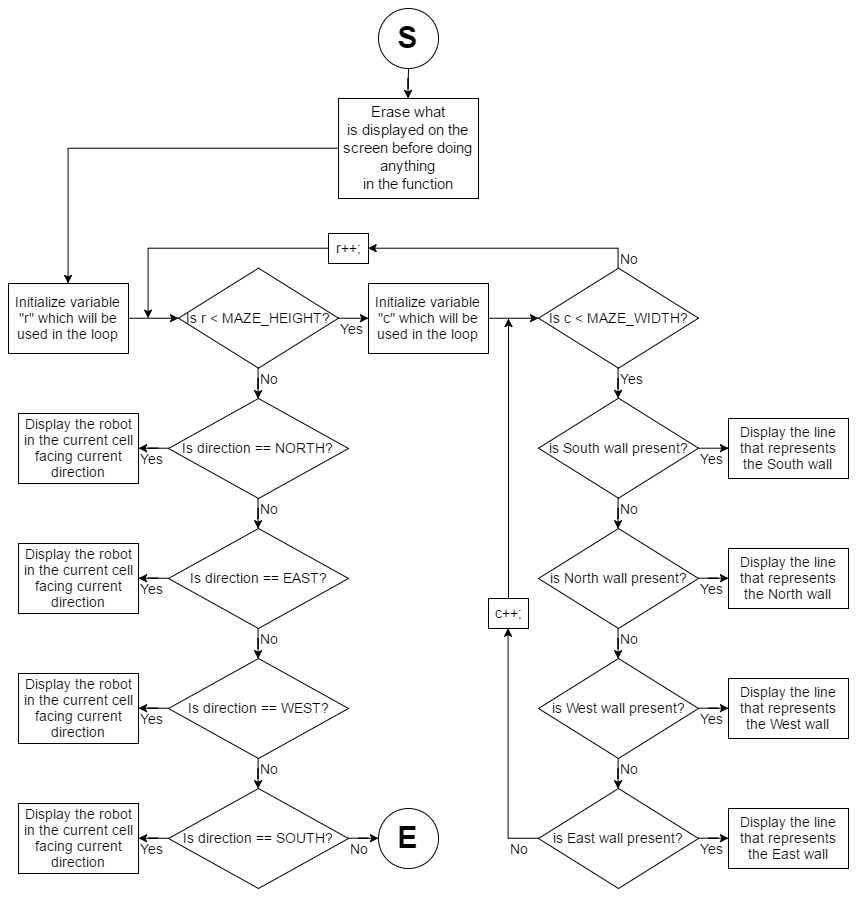
\includegraphics[scale=0.516]{images/Software_Flowchart/Drawing_Function.png}
\caption{Flow Chart for Displaying Function}
\label{}
\end{figure}
	\begin{itemize}
	\item The local variable direction is passed into the function but it does not return any variable
	\item Global variables and constants used are
	\begin{verbatim}
		MAZE_WIDTH
		MAZE_HEIGHT
		CELL_WIDTH
		CELL_HEIGHT
		CELL_WIDTH_MIDDLE
		CELL_HEIGHT_MIDDLE
	\end{verbatim}
	\end{itemize}
\end{itemize}
\newpage

%% 3.8

\subsection{Moving Forward Function}
\begin{itemize}
\item Function to draw current informations of the robot on the screen
	\begin{verbatim}
		void goFwdCell(int direction);
	\end{verbatim}
\begin{figure}[htp]
\centering
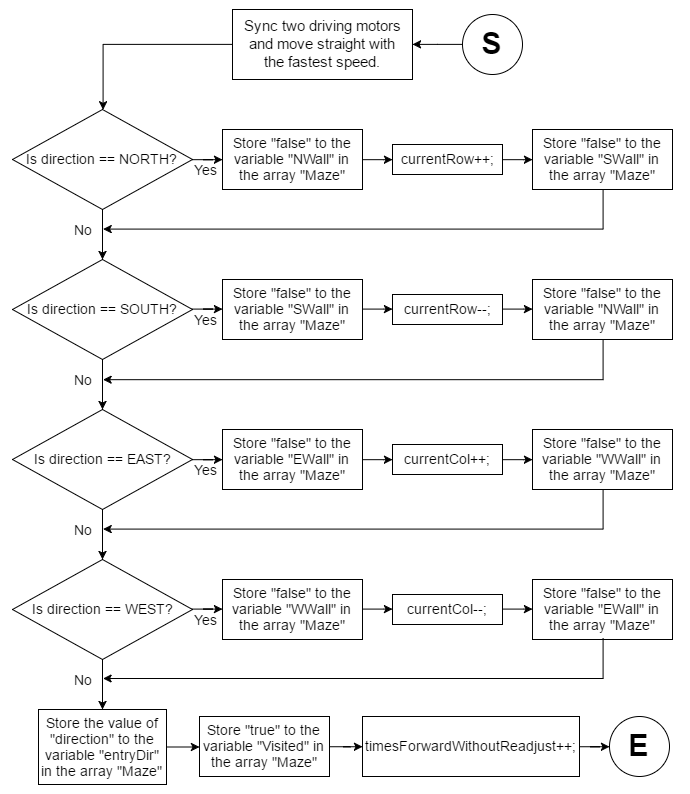
\includegraphics[scale=0.56]{images/Software_Flowchart/Moving_Forward.png}
\caption{Flow Chart for Moving Forward}
\label{}
\end{figure}	
	\begin{itemize}
	\item The local variable direction is passed into the function but it does not return any variable
	\item Global variables and constants used are
	\begin{verbatim}
		SIZE_OF_ONE_CELL
		CIRCUMFERENCE_OF_WHEEL
		DRIVE_GEAR_RATIO
		ONE_ROTATION
		FORWARD
		timesForwardWithoutReadjust
	\end{verbatim}
	\end{itemize}
\end{itemize}
\newpage

%% 3.9

\subsection{Turning Functions}
\begin{itemize}
\item Function for Turning right
\begin{verbatim}
	int Turn90CW(int direction);
\end{verbatim}
\begin{figure}[htp]
\centering
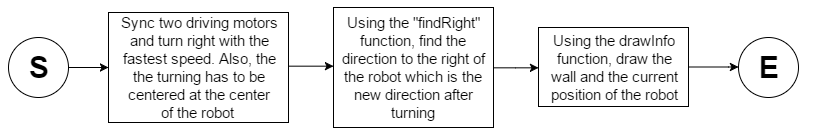
\includegraphics[scale=0.6]{images/Software_Flowchart/Turning_Right.png}
\caption{Flow Chart for Turning Right}
\label{}
\end{figure}
	\begin{itemize}
	\item The local variable direction is passed into the function and it returns the same variable direction
	\item Global variables and constants used are
	\begin{verbatim}
		QUARTER_ROTATION;
		DRIVE_GEAR_RATIO;
		FORWARD;
	\end{verbatim}
	\item This function calls in other functions
	\begin{verbatim}
		int findRight(int direction);
		int drawInfo(int direction);
	\end{verbatim}
	\end{itemize}
\item Function for Turning left 
\begin{verbatim}
	Turn90CW(int direction);
\end{verbatim}
\begin{figure}[htp]
\centering
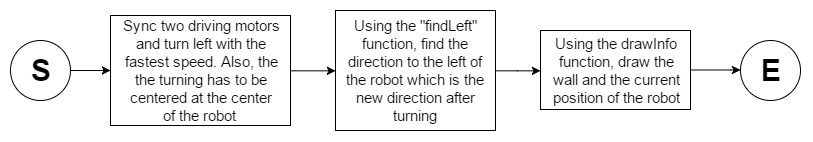
\includegraphics[scale=0.60]{images/Software_Flowchart/Turning_Left.png}
\caption{Flow Chart for Turning Left}
\label{}
\end{figure}
	\begin{itemize}
	\item The local variable direction is passes into the function and it returns the same variable direction
	\item Global variables and constants used are
	\begin{verbatim}
		QUARTER_ROTATION;
		DRIVE_GEAR_RATIO;
		FORWARD;
	\end{verbatim}
	\item This function calls in other functions
	\begin{verbatim}
		int findLeft(int direction);
		int drawInfo(int direction);
	\end{verbatim}
	\end{itemize}
\end{itemize}
\newpage

%% 3.10

\subsection{Wall Detecting Function}
\begin{itemize}
\item Function that detects wall with the sensor
	\begin{verbatim}
		int thereIsWall();
	\end{verbatim}
\begin{figure}[htp]
\centering
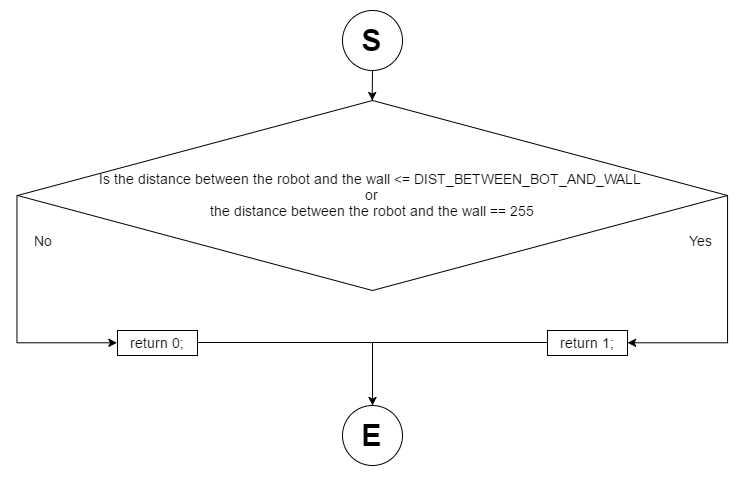
\includegraphics[scale=0.60]{images/Software_Flowchart/Detecting_Wall.png}
\caption{Flow Chart for Wall Detecting Function}
\label{}
\end{figure}
	\begin{itemize}
	\item Very simple fuction that returns $1$ if the sensor detects the wall
	\item Global variables and constants used are
	\begin{verbatim}
		DIST_BETWEEN_BOT_AND_WALL
	\end{verbatim}
	\end{itemize}
\end{itemize}
\newpage

%% 3.11

\subsection{Function for Storing Data of the Walls}
\begin{itemize}
\item Function that stores data of the walls to the variables
	\begin{verbatim}
		void writeWall(int direction);
	\end{verbatim}
\begin{figure}[htp]
\centering
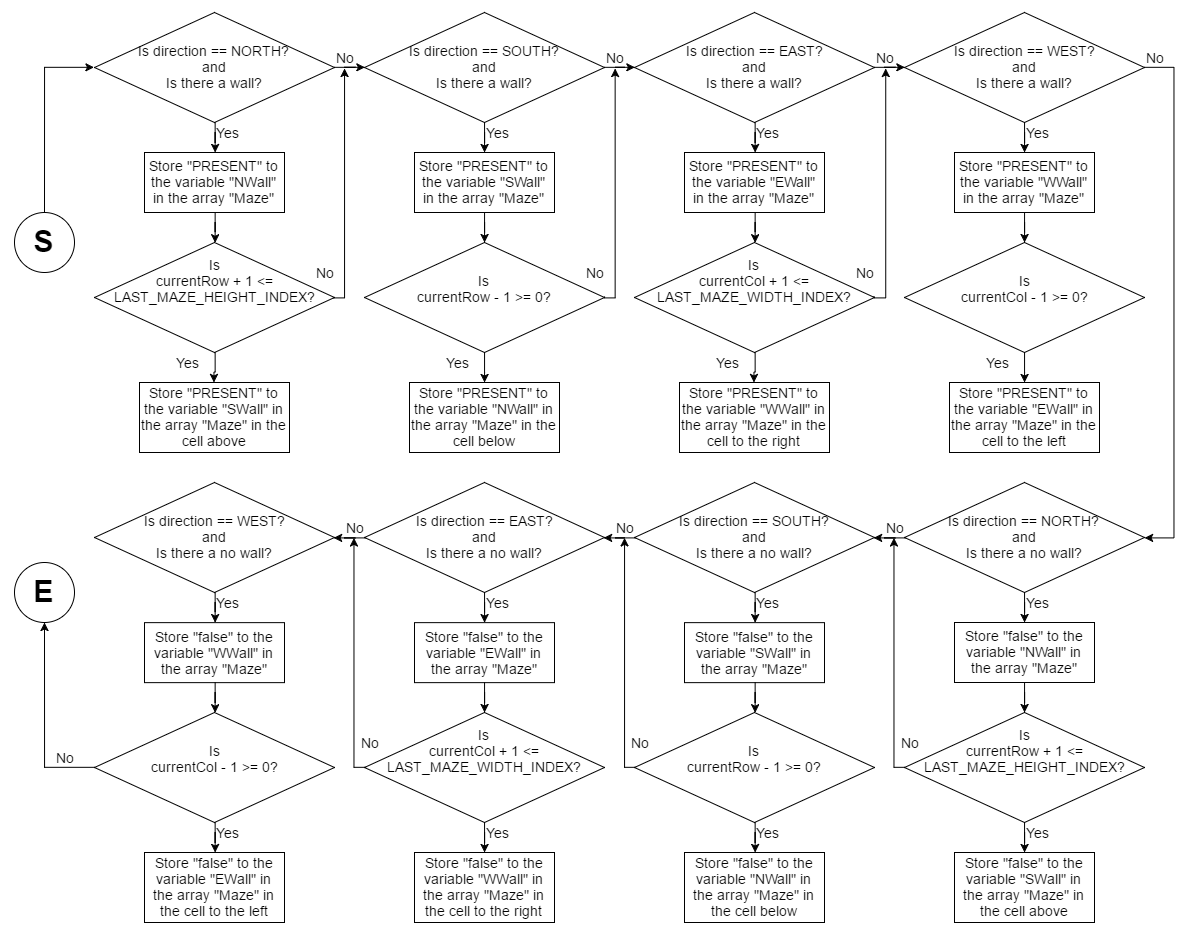
\includegraphics[scale=0.41]{images/Software_Flowchart/writeWall.png}
\caption{Flow Chart for Storing Data Function}
\label{}
\end{figure}
	\begin{itemize}
	\item The local variable direction is passed into the function but it does not return any variable
	\item Global variables and constants used are
	\begin{verbatim}
		NORTH
		SOUTH
		EAST
		WEST
		currentRow
		currentCol
		PRESENT
		LAST_MAZE_HEIGHT_INDEX
		LAST_MAZE_WIDTH_INDEX
	\end{verbatim}
	\item This function calls in other functions 
	\begin{verbatim}
		int thereIsWall();
	\end{verbatim}
	\end{itemize}
\end{itemize}
\newpage

%% 3.12

\subsection{Functions for setting up the direction that need to be used}
\begin{itemize}
\item Function that takes in the current direction of the robot and returns exact opposite direction of what the robot is facing
	\begin{verbatim}
		int findBackDir(int currentDirection);
	\end{verbatim}
\begin{figure}[htp]
\centering
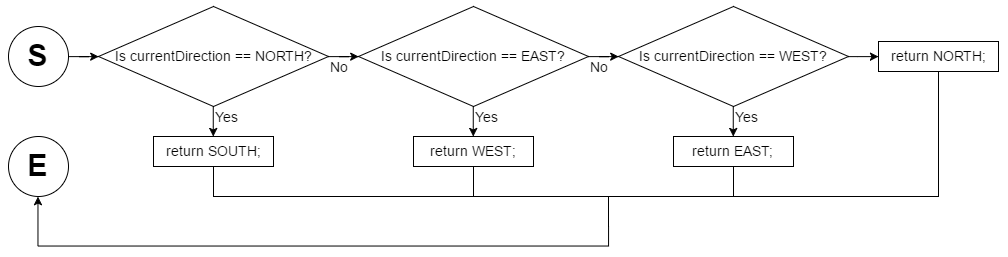
\includegraphics[scale=0.45]{images/Software_Flowchart/findBackDir.png}
\caption{Flow Chart for Finding Back Function}
\label{}
\end{figure}
\item Function that takes in the current direction of the robot and returns the right direction of the robot
	\begin{verbatim}
		int findRight(int currentDirection);
	\end{verbatim}
\begin{figure}[htp]
\centering
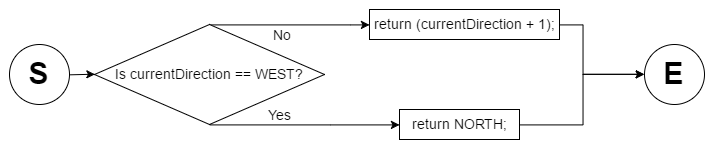
\includegraphics[scale=0.47]{images/Software_Flowchart/findRight.png}
\caption{Flow Chart for Finding Right Function}
\label{}
\end{figure}	
\item Function that takes in the current direction of the robot and returns the left direction of the robot
	\begin{verbatim}
		int findLeft(int currentDirection);
	\end{verbatim}
\begin{figure}[htp]
\centering
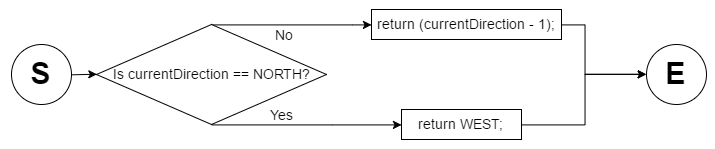
\includegraphics[scale=0.48]{images/Software_Flowchart/findLeft.png}
\caption{Flow Chart for Finding Left Function}
\label{}
\end{figure}
	\begin{itemize}
	\item Global variables and constants used are
	\begin{verbatim}
		NORTH
		SOUTH
		EAST
		WEST
	\end{verbatim}
	\end{itemize}
\end{itemize}
\newpage

%% 3.13

\subsection{Functions for Finding Existence of Wall from the data}
\begin{itemize}
\item Function that uses the data saved from detecting function
	\begin{verbatim}
		int isThereWallInDir(int wallDir);
	\end{verbatim}
\begin{figure}[htp]
\centering
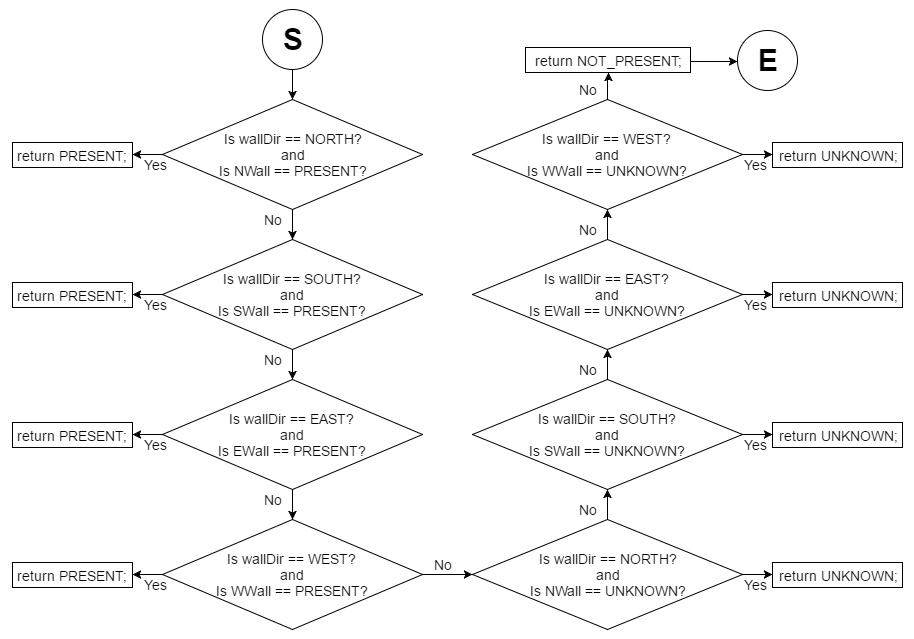
\includegraphics[scale=0.580]{images/Software_Flowchart/isThereWallInDir.png}
\caption{Flow Chart for Finding Existence of Wall from the data}
\label{}
\end{figure}
	\begin{itemize}
	\item Global variables and constants used are
	\begin{verbatim}
		NORTH
		SOUTH
		EAST
		WEST
		PRESENT
		UNKNOWN
		NOT_PRESENT
	\end{verbatim}
	\end{itemize}
\end{itemize}
\newpage

%% 3.14

\subsection{Functions for Readjusting in Certain Directions}
\begin{itemize}
\item Function that readjusts robot's direction by moving towards the wall and comes back to the center of the cell. For this function particularly, we readjust using walls to the front and to the right.
	\begin{verbatim}
		void reAdjustCW(int direction);
	\end{verbatim}
\begin{figure}[htp]
\centering
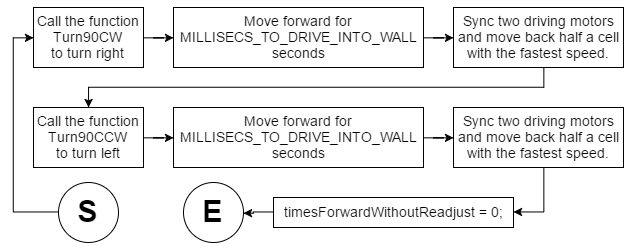
\includegraphics[scale=0.52]{images/Software_Flowchart/reAdjustCW.png}
\caption{Flow Chart for Readjusting using Front wall and Right wall}
\label{}
\end{figure}
\item Function that readjusts robot's direction by moving towards the wall and comes back to the center of the cell. For this function particularly, we readjust using walls to the front and to the left.
	\begin{verbatim}
		void reAdjustCCW(int direction);
	\end{verbatim}
\begin{figure}[htp]
\centering
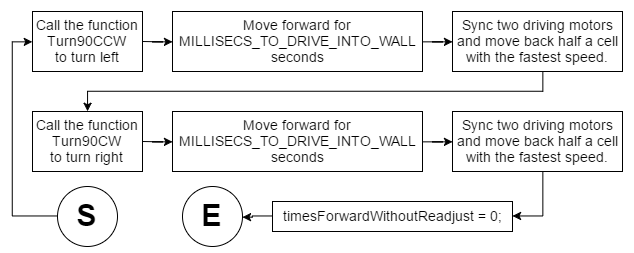
\includegraphics[scale=0.52]{images/Software_Flowchart/reAdjustCCW.png}
\caption{Flow Chart for Readjusting using Front wall and Left wall}
\label{}
\end{figure}
	\begin{itemize}
	\item The local variable direction is passed into the function but it does not return any variable
	\item Global variables and constants used are
	\begin{verbatim}
		FORWARD
		BACKWARD
		SIZE_OF_ONE_CELL
		CIRCUMFERENCE_OF_WHEEL
		DRIVE_GEAR_RATIO
		ONE_ROTATION
		UNCERTAINTY_READJUST
		MILLISECS_TO_DRIVE_INTO_WALL
	\end{verbatim}
	\item This function calls in other functions
	\begin{verbatim}
		int Turn90CW(int direction);
		int Turn90CCW(int direction);
	\end{verbatim}
	\end{itemize}
\newpage
\item Function that readjusts robot's direction by moving towards the wall and comes back to the center of the cell. With this Function, the robot uses the saved data to determine to readjust in CW direction or CCW direction
	\begin{verbatim}
		void reAdjustWayBack(int direction);
	\end{verbatim}
\begin{figure}[htp]
\centering
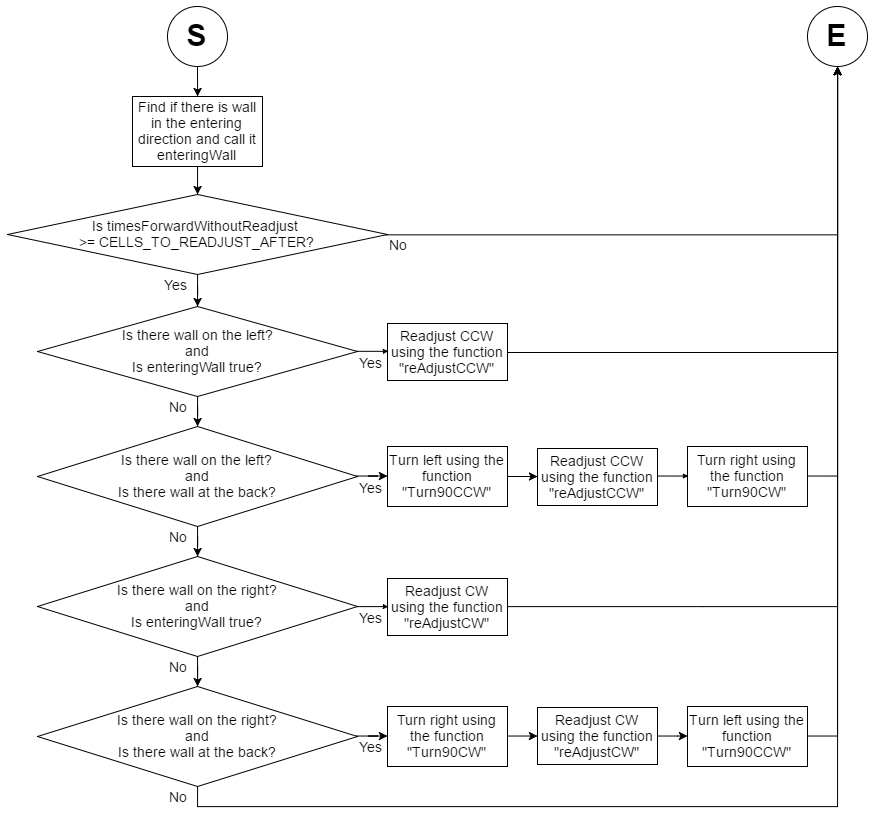
\includegraphics[scale=0.46]{images/Software_Flowchart/reAdjustWayBack.png}
\caption{Flow Chart for Readjusting using walls detected}
\label{}
\end{figure}
	\begin{itemize}
	\item The local variable direction is passed into the function but it does not return any variable
	\item Global variables and constants used are
	\begin{verbatim}
		timesForwardWithoutReadjust
		CELLS_TO_READJUST_AFTER
		PRESENT
	\end{verbatim}
	\item This function calls in other functions
	\begin{verbatim}
		thereIsWall();
		reAdjustCW(int direction);
		reAdjustCCW(int direction);
		findLeft(int currentDirection);
		findRight(int currentDirection);
		findBackDir(int currentDirection);
		isThereWallInDir(int wallDir);
	\end{verbatim}
	\end{itemize}
\end{itemize}
\newpage

%% 3.15

\subsection{Function for Movement All Together}
\begin{itemize}
\item Function that contains all other smaller functions for movement and this is the only function called in the main task
	\begin{verbatim}
		int MovementWithSensor(int direction);
	\end{verbatim}
\begin{figure}[htp]
\centering
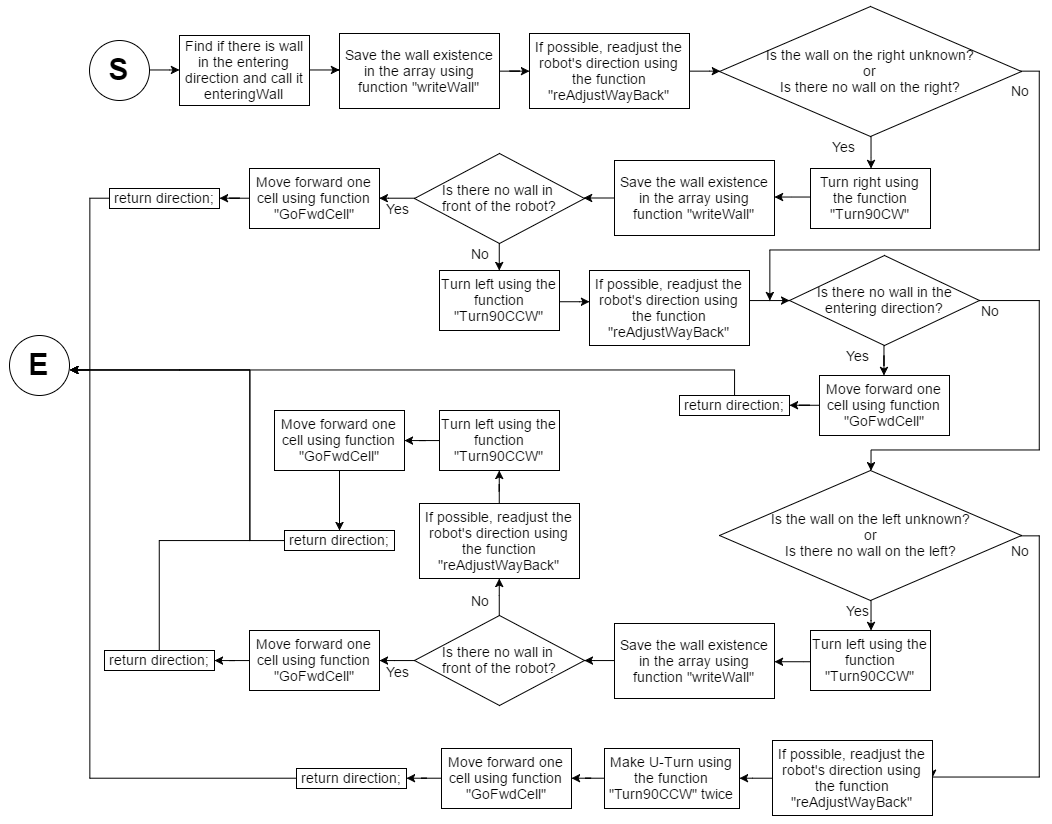
\includegraphics[scale=0.45]{images/Software_Flowchart/MovementWithSensor.png}
\caption{Flow Chart for Movement Function}
\label{}
\end{figure}
	\begin{itemize}
	\item The local variable direction is passed into the function and it returns the same variable direction
	\item Global variables and constants used are
	\begin{verbatim}
		UNKNOWN
		NOT_PRESENT
	\end{verbatim}
	\item This function calls in other functions
	\begin{verbatim}
		writewall(int direction);
		reAdjustWayBack(int direction);
		isThereWallInDir(int wallDir);
		findRight(int currentDirection);
		thereIsWall();
		goFwdCell(int direction);
		Turn90CCW(int direction);
		Turn90CW(int direction);
	\end{verbatim}
	\end{itemize}
\end{itemize}
\newpage

%% 3.16

\subsection{Functions for Returning Algorithm}
\begin{itemize}
\item Function that deletes the duplicates from the array which saved up how the robot entered each cell. For example, if the robot moved two opposite directions in order, it is not necessary. Therefore, we delete the duplicates from the array
 	\begin{verbatim}
		void deleteDuplicates();
	\end{verbatim}
\begin{figure}[htp]
\centering
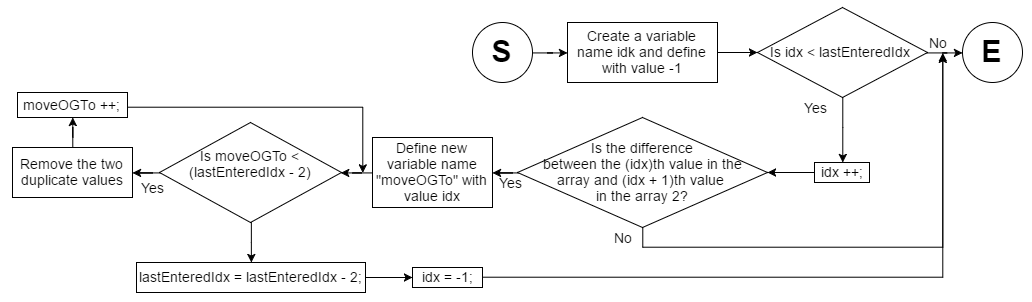
\includegraphics[scale=0.50]{images/Software_Flowchart/deleteDuplicate.png}
\caption{Flow Chart for Deleting Duplicate Function}
\label{}
\end{figure}
\item Function that reverses the direction from the array which saved up how the robot entered each cell. For example, if the robot went in to the cell with direction East, then we change it to West. Therefore, we change all the directions to its opposite.
 	\begin{verbatim}
		void reverseDirection();
	\end{verbatim}
\begin{figure}[htp]
\centering
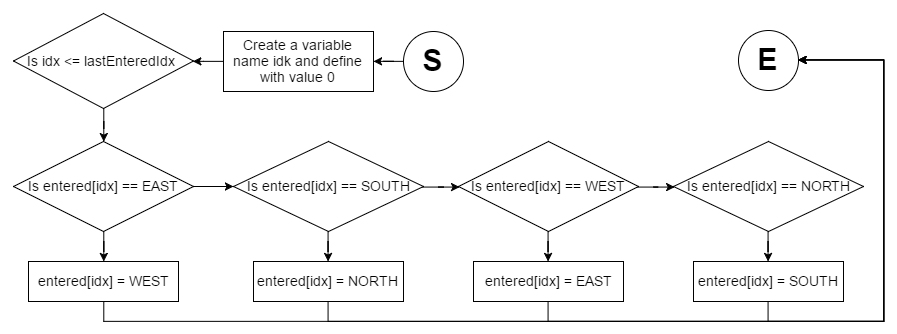
\includegraphics[scale=0.50]{images/Software_Flowchart/reverseDirection.png}
\caption{Flow Chart for Reversing Order of Values in the Array}
\label{}
\end{figure}
\newpage
\item Function that takes in the variable direction and goes back to the initial position in the cell with the new array created by two functions above
 	\begin{verbatim}
		void goingBackFastestRoute(int direction);
	\end{verbatim}
\begin{figure}[htp]
\centering
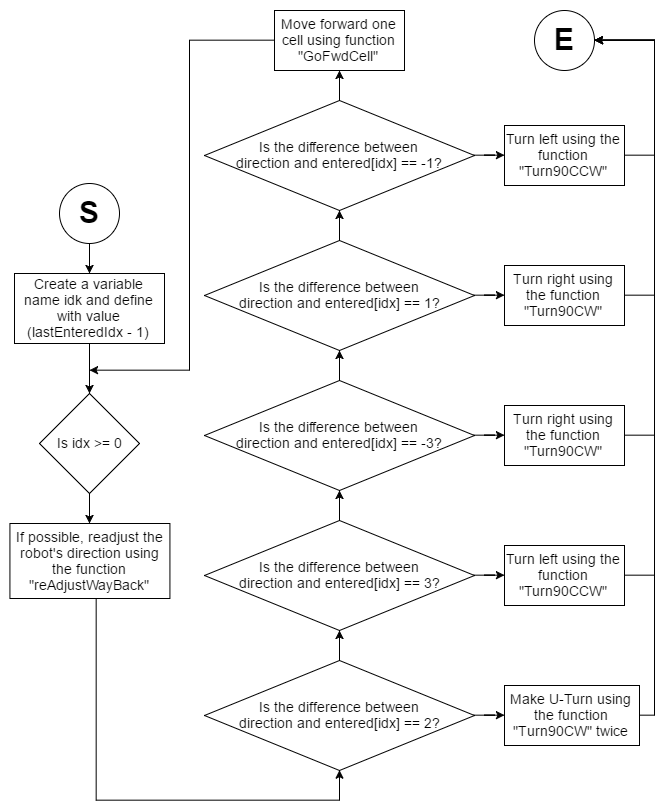
\includegraphics[scale=0.53]{images/Software_Flowchart/goingBackFastestRoute.png}
\caption{Flow Chart for Function to Go Back to Initial Position}
\label{}
\end{figure}
	\begin{itemize}
	\item Global variables and constants used are
	\begin{verbatim}
		lastEnteredIdx
		EAST
		WEST
		SOUTH
		NORTH
	\end{verbatim}
	\item This function calls in other functions
	\begin{verbatim}
		reAdjustWayBack(int direction);	
		Turn90CW(int direction);
		Turn90CCW(int direction);
	\end{verbatim}
	\end{itemize}
\end{itemize}
\newpage

%% 3.17

\subsection{Main Function}
\begin{itemize}
\item More than ten functions were declared for simplicity of the main function. This function sums up all smaller functions
	\begin{verbatim}
		task main()
	\end{verbatim}
\begin{figure}[htp]
\centering
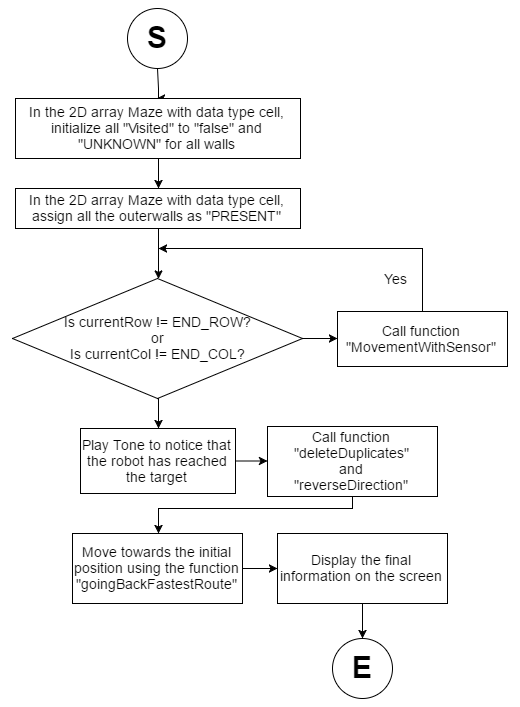
\includegraphics[scale=0.51]{images/Software_Flowchart/task_main.png}
\caption{Flow Chart of the Main Function}
\label{}
\end{figure} 
	\begin{itemize}
	\item Global variables and constants used are
	\begin{verbatim}
		MAZE_WIDTH
		MAZE_HEIGHT
		UNKNOWN
		PRESENT
		lastEnteredIdx
		FREQUENCY
		MILI_TO_BEEP_FOR
	\end{verbatim}
	\item This function calls in other functions
	\begin{verbatim}
		MovmentWithSensor(int direction);
		deleteDuplicates();
		reverseDirection();
		goingBackFastestRoute(int direction);
		drawInfo(int direction);
	\end{verbatim}
	\end{itemize}
 

\end{itemize}

\newpage

%% Do not remove the gap %%








\section{Appendix}

Source of Code with brief comments


\end{document}
